\subsection{Complexity}
\label{s:IDC:Complex}
When worrying about complexity in an experiment, a widely abused
aphorism (sometimes attributed to Einstein) comes to mind: 
``Everything should be made as simple as possible, but not simpler.''
The interferometer design should be made as simple as possible, but not so simple as to degrade the controllability and sensitivity.
In Figure~\ref{fig:IDC:SensEvo}, the evolution of the strain sensitivity is plotted
versus time. The noise hunting~\cite{Rana:PhD} of the interferometer began in earnest at the
point when the two arm cavities were brought into simultaneous resonance. As is
clear, the noise reduction in the case of Advanced LIGO has been much more rapid
than in the initial detectors. What are the reasons for this? There are two chief
factors: a more experienced interferometer commissioning team and a more expensive
and complicated interferometer design.

\begin{figure}[h]
\centering
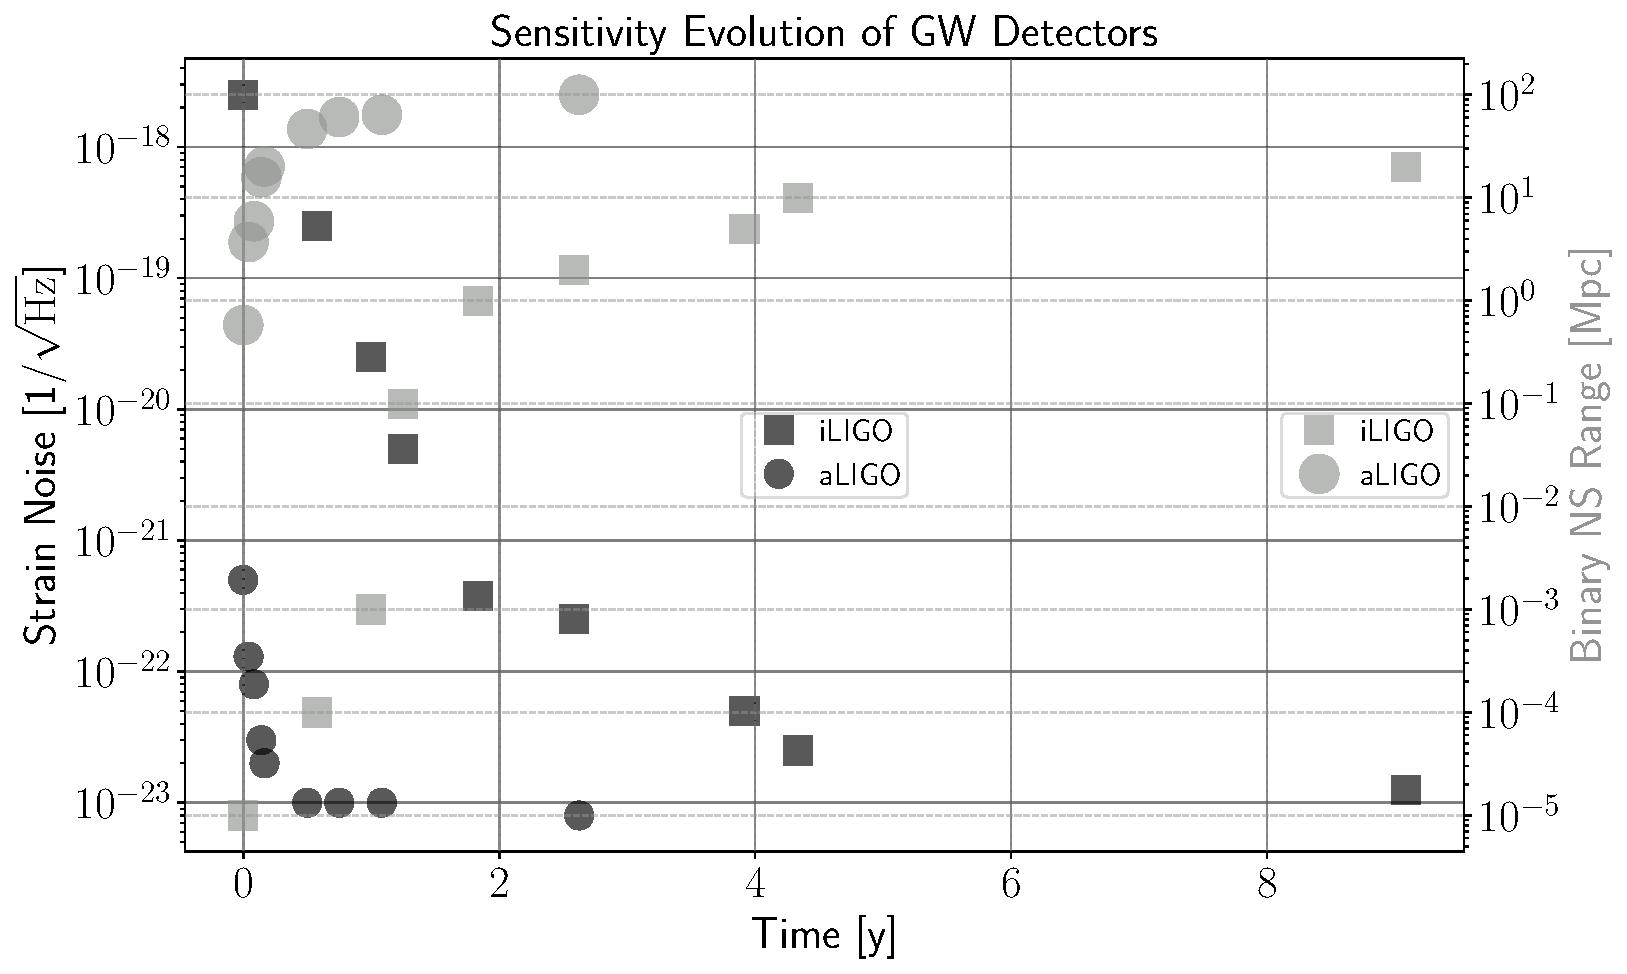
\includegraphics[width=\columnwidth]{Figures/NoiseProgComp.pdf}
\caption{Evolution of the interferometer strain sensitivities. The $t = 0$
  point is chosen, in each case, to coincide with the first time that the
  two arms are brought into resonance. The circle and star show the evolution of
  the binary neutron star inspiral reach and the square and the pentagon show
  the reduction in the strain noise spectral density.}
\label{fig:IDC:SensEvo}
\end{figure}

A great deal of emphasis is often placed on making the system design 'simple'
(a phrase which seems to have different meanings to everyone). A great
experiment should be designed to be as simple as possible, but no more so. We have
seen that the initial generation of detector was made too simple; passive vibration
isolation using tables made of rubber and steel, single stage pendulums holding
the mirrors, and no adaptive optics. The complicated vibration isolation system,
which includes N sensors and N feedback loops (cf. Chapter~\ref{SEI})
reduces the seismic motions of the interferometer mirrors by
orders of magnitude (compare the 0.1\,--\,3\,Hz transfer functions of AdvLIGO/Virgo with GEO600, initial LIGO, and TAMA SAS). The
complicated multiple stage pendulum Virgo, GEO600, and Adv. LIGO
allows the remaining seismic motion to be allocated intelligently
among the different stages, such that the actuators in the final stages
may be weak and inject less noise. By integrating the thermal wavefront
compensation systems (cf.~\ref{TCS}) in the baseline design, the
interferometers can be made to operate stably with any operating power,
whereas the first generation interferometers suffered from a lack of optical stability at all but a narrow range of operating power levels.

The addition of hundreds of sensors and feedback loops, along with more careful
optical modeling, has lead to a more 'simple' system from the standpoint of
detector commissioning and has reduced the time between installation and astrophysical data taking. The information earned by fighting with first generation of interferometers has yielded valuable fruits and one can only assume that we are now sowing the seeds for the third generation to reap.

\begin{figure}[h]
\centering
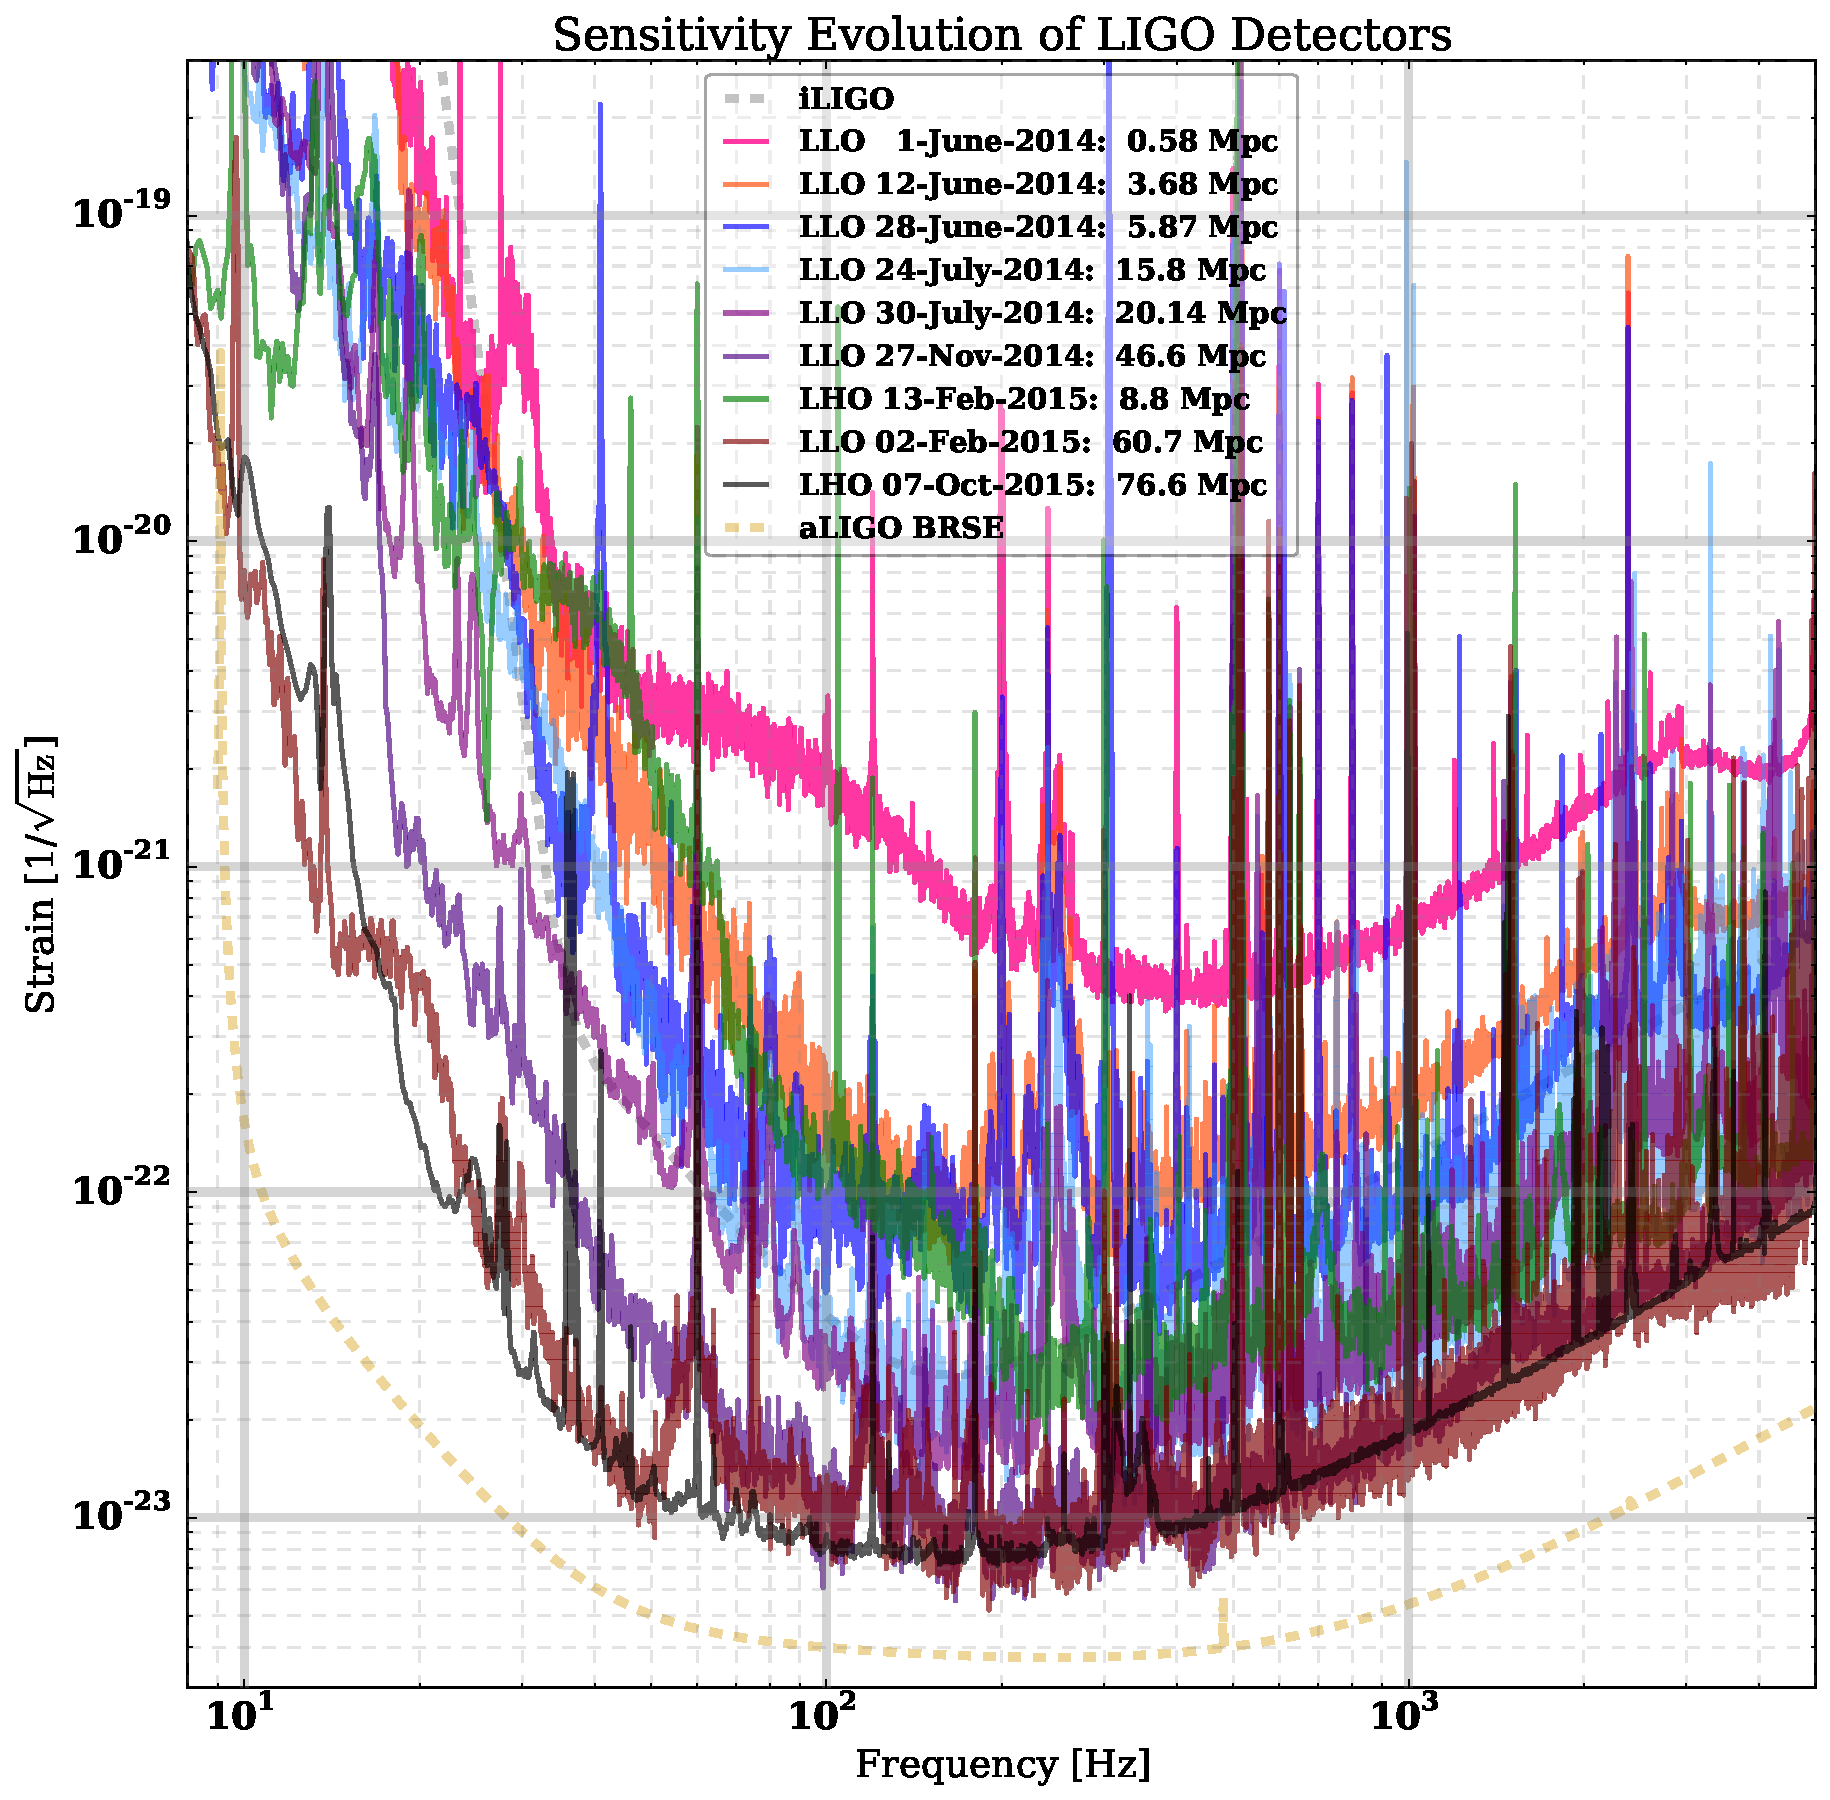
\includegraphics[width=\columnwidth]{Figures/aLIGO_noises.pdf}
\caption{Strain noise reduction of the Advanced LIGO interferometers
  through 2016.}
\label{fig:IDC:aLIGOnoises}
\end{figure}
